% !TEX root = ../waves.tex
In the previous chapter, we demonstrated that under favourable conditions, periodic
functions can be written as an infinite series of elementary trigonometric functions, the
Fourier series. This expansion is crucial for studying oscillatory phenomena, as it
decomposes any oscillating function into a sum of pure sine and cosine waves. Another
crucial property presented in~\cref{eq:cn-der} is that the Fourier coefficients of the
derivative of a function $f$ are simply the coefficients of $f$ multiplied by a power of
the frequency. This property is quite powerful as it can transform linear differential
equations into simpler polynomial equations. However, the Fourier series expansion is in
principle limited to describing periodic functions, and one can legitimately wonder if it
can be generalised to non-periodic functions.

A first interesting observation is that Fourier series can be used to represent
non-periodic functions on any finite interval. Indeed, let us consider a function $f$ on
$\R$, which we consider smooth for the sake of simplicity. Let $A$ be a positive real
number, then according to~\cref{thm:fourier-pt}, for all $x\in(-A,A)$,
\begin{equation}
  f(x)=\sumz{n}c_n\,e^{\frac{\pi}{A}inx}\,,\label{eq:series-nonper}
\end{equation}
with the Fourier coefficients
\begin{equation}
  c_n=\frac{1}{2A}\int_{-A}^{A}\diff x\,f(x)\,e^{-\frac{\pi}{A}inx}\,.\label{eq:cn-nonper}
\end{equation}
This happens because $f$ restricted to $(-A,A)$ can be interpreted as one period of a
$2A$-periodic function $\bar{f}$ defined by $\bar{f}=f$ on $(-A,A)$. Outside $(-A,A)$, the
series~\cref{eq:series-nonper} converges to a periodic copy of $f$ in $(-A,A)$.
Interestingly, this can be done for arbitrarily large $A$, and one can question whether
the whole function $f$ on $\R$ can be described in that way by taking the $A\to+\infty$
limit. We can try to formally conjecture what such a limit would look like, ignoring for
the moment potential convergence issues. We start by recalling the rectangle approximation
for an integral
\begin{equation}
  \lim_{a\to0}\,\sumz{n}a\,F(an)=\int_{-\infty}^{+\infty}\diff x\, F(x)\,,
\end{equation}
where $F$ is an integrable function on $\R$. Using this formula with $a=\frac{1}{2A}$, one
can conjecture that the $A\to+\infty$ limit of~\cref{eq:series-nonper} leads to
\begin{equation}
  \label{eq:ft-conjecture}
  f(x)=\int_{-\infty}^{+\infty}\diff\omega\,\hat{f}(\omega)\,e^{2\pi i\omega x},
  \qquad\text{with}\qquad
  \hat{f}(\omega)=\int_{-\infty}^{+\infty}\diff x\,f(x)\,e^{-2\pi i\omega x}\,.
\end{equation}
So on an infinite range, the Fourier coefficient index $n$ becomes a continuous variable.
The associated function $\hat{f}$ is called the \emph{Fourier transform} of $f$, and $f$
and $\hat{f}$ have an interesting duality through the relationships above. This duality is
absolutely fundamental both in physics and mathematics, and can be seen as a
generalisation of Fourier series. Clearly, many things can go wrong when taking the
$A\to+\infty$ limit above, and one needs to derive the formulas above more carefully. It
can be shown that the Fourier transform can be defined for a remarkably wide range of
mathematical objects. However, its proper construction relies on technical knowledge of
functional analysis and integration theory, going beyond the scope of this introductory
course. Therefore, this chapter is mostly aimed at explaining how to use Fourier
transforms practically, and results will often have part of their proof admitted.

We start by defining the Fourier transform and studying its properties for a simple class
of functions for which the integrals above are clearly defined.
%%%%%%%%%%%%%%%%%%%%%%%%%%%%%%%%%%%%%%%%%%%%%%%%%%%%%%%%%%%%%%%%%%%%%%%%%%%%%%%%%%%%%%%%%%
\section{Fourier transform of Schwartz functions}
As we discussed in the case of Fourier series,
particularly~\cref{thm:fourier-series-decay}, there is a connection between the smoothness
of a function and the decay rate of its Fourier coefficients. So, unsurprisingly, a good
starting point to build the Fourier transform is to define a class of very smooth and
rapidly decaying functions, which are the Schwartz functions.
%-----------------------------------------------------------------------------------------
\subsection{Definition and properties}
We start by defining two classes of functions based on their decay rates.
\begin{definition}
  A function $f$ on $\R$ is called a \emph{rapidly decaying function} if it decays faster
  than any power at infinity. Explicitly, for all non-negative integers $\alpha$,
  \begin{equation}
    \lim_{|x|\to+\infty}x^\alpha f(x)=0\,.
  \end{equation}
\end{definition}
\begin{definition}
  A function $f$ on $\R$ is called a \emph{moderately growing function} if it does not
  grow faster than a given power. Explicitly, there exists a non-negative integer $\alpha$
  such that
  \begin{equation}
    \lim_{|x|\to+\infty}x^{-\alpha}f(x)=0\,.
  \end{equation}
\end{definition}
The key idea here is that if a function is rapidly decaying, multiplying it by a
moderately growing function will not change that, which will be useful when considering
dot products of functions.
\begin{proposition}
  \label{prop:rapid-times-moderate}
  All rapidly decaying functions on $\R$ are moderately growing. The product of a rapidly
  decaying function and a moderately growing function is a rapidly decaying function.
\end{proposition}
\begin{proof}
  Let $f$ be a rapidly decaying function on $\R$, and $g$ a moderately growing function on
  $\R$. Then there exists a non-negative integer $\alpha$ such that
  \begin{equation}
    \lim_{|x|\to+\infty}x^{-\alpha}g(x)=0\,.
  \end{equation}
  Let $\beta$ be a non-negative integer, then
  \begin{equation}
    \lim_{|x|\to+\infty}x^\beta f(x)g(x)=
    \lim_{|x|\to+\infty}[x^{\alpha+\beta} f(x)][x^{-\alpha}g(x)]=0\,,
  \end{equation}
  so $fg$ is a rapidly decaying function.
\end{proof}
We now define Schwartz functions:
\begin{definition}
  \label{def:schwartz-fn}
  A function $f$ on $\R$ is called a \emph{Schwartz function} if it is infinitely
  differentiable, and if $f$ and all its derivatives are rapidly decaying functions. More
  explicitly, for all pairs of non-negative integers $\alpha$ and $\beta$,
  \begin{equation}
    \lim_{|x|\to+\infty}x^\beta f^{(\alpha)}(x)=0\,.
  \end{equation}
\end{definition}
We then have the two propositions below regarding simple combinations of Schwartz
functions. The proofs are fairly straightforward and left as an exercise to the reader.
\begin{proposition}
  \label{prop:schwartz-comb}
  An arbitrary linear combination of Schwartz functions is a Schwartz function. A product
  of Schwartz functions is also a Schwartz function. A derivative of a Schwartz function
  is a Schwartz function.
\end{proposition}
\begin{proposition}
  Let $f$ be a Schwartz function on $\R$, and $g$ be an infinitely differentiable function
  of moderate growth. Then the product $fg$ is a Schwartz function.
\end{proposition}
Let us now discuss some examples and counter-examples. A crucial example of a Schwartz
function is the Gaussian kernel.
\begin{definition}
  \label{def:gauss}
  We call \emph{Gaussian kernel} with \emph{width} $\sigma$ the function $\gauss_{\sigma}$
  defined on $\R$ by
  \begin{equation}
    \gauss_{\sigma}(x)=\frac{1}{\sigma\sqrt{2\pi}}\,e^{-\frac{x^2}{2\sigma^2}}\,,
  \end{equation}
  where $\sigma$ is a positive real number.
\end{definition}
\begin{proposition}
  \label{prop:gauss-schwartz}
  The Gaussian kernel $\gauss_{\sigma}$ is a Schwartz function.
\end{proposition}
\begin{proof}
  This proof is part of the exercises of this chapter.
\end{proof}
The Gaussian kernel is illustrated in~\cref{fig:gauss}. It is a function peaked at zero
for small widths. A well-known result, particularly in statistics, is that for a given
width $\sigma$, approximately $68.3\%$ of the area under the curve of $\gauss_{\sigma}$ is
in the interval $[-\sigma,\sigma]$, and $95\%$ is in the interval $[-2\sigma,2\sigma]$.
\begin{figure}[t]
  \centering
  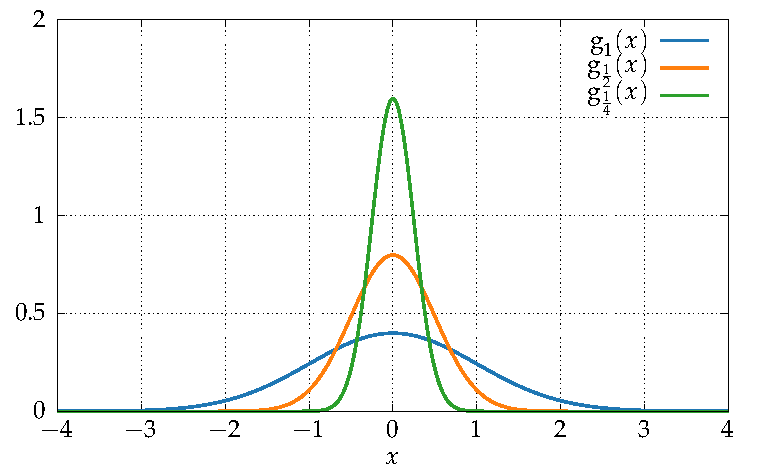
\includegraphics{gp_gauss.pdf}
  \caption{Curve of the Gaussian kernel defined in \cref{def:gauss} for several widths.}
  \label{fig:gauss}
\end{figure}
\begin{example}
  The function $f$ defined for $x\in\R$ by
  \begin{equation}
    f(x)=\frac{1}{x^2+2}\,,
  \end{equation}
  is not a Schwartz function, although it is infinitely differentiable. Indeed,
  \begin{equation}
    \lim_{x\to+\infty} x^2\,f(x)=1\,,
  \end{equation}
  which does not satisfy~\cref{def:schwartz-fn}. It is, however, a function of moderate
  growth.
\end{example}
\begin{example}
  The function $f$ defined for $x\in\R$ by
  \begin{equation}
    f(x)=e^{-|x|}\,,
  \end{equation}
  is not a Schwartz function, although it is a rapidly decaying function. Indeed,
  \begin{equation}
    f'(x)=-\sign(x)\,e^{-|x|}\,,
  \end{equation}
  is discontinuous at $0$, and therefore $f$ does not admit a second derivative.
\end{example}
\begin{example}
  All polynomials are functions of moderate growth, but the exponential function is not a
  function of moderate growth.
\end{example}
We also generalise the dot product introduced in~\cref{def:func-dot}
\begin{definition}
  Let $f$ be a Schwartz function on $\R$, and $g$ be an integrable moderately growing
  function on $\R$. We define the \emph{dot product} $\braket{f,g}$ of $f$ and $g$ with
  the following integral
  \begin{equation}
    \braket{f,g}=\intr{x}f(x)g(x)^*\,.
  \end{equation}
  Additionally, the norm $\|f\|$ of a Schwartz function $f$ is defined by
  \begin{equation}
    \|f\|^2=\braket{f,f}=\intr{x}|f(x)|^2
  \end{equation}
\end{definition}
It is important to note that the norm of a moderately growing function and the dot product
of two moderately growing functions are generally not well-defined, as the associated
integrals might not converge. Schwartz functions have the following simple integration by
parts formula.
\begin{proposition}
  \label{prop:schwartz-partint}
  Let $f$ be a Schwartz function on $\R$, and let $g$ be a continuously differentiable
  function of moderate growth. Then we have the integration by parts formula
  \begin{equation}
    \intr{x}f'(x)g(x)=-\intr{x}f(x)g'(x)\,.
  \end{equation}
  Or, equivalently, $\braket{f',g}=-\braket{f,g'}$.
\end{proposition}
\begin{proof}
  Let $A$ be a positive real number, we have
  \begin{equation}
    \int_{-A}^A\diff x\,f'(x)g(x)=[f(x)g(x)]_{-A}^A-\int_{-A}^A\diff x\,f(x)g'(x)\,.
  \end{equation}
  Using \cref{prop:rapid-times-moderate}, $fg$ is a rapidly decaying function so
  \begin{equation}
    \lim_{A\to+\infty}[f(x)g(x)]_{-A}^A=0\,.
  \end{equation}
  Taking the same limit in the two integrals above proves the proposition.
\end{proof}
We are now ready to define the Fourier transform:
\begin{definition}
  Let $f$ be an integrable function on $\R$, the function $\hat{f}$ defined on $\R$ by
  \begin{equation}
    \hat{f}(\omega)=\int_{-\infty}^{+\infty}\diff x\,f(x)\,e^{-2\pi i\omega x}\,,
  \end{equation}
  is called the \emph{Fourier transform} of $f$. We additionally note $\mathcal{F}$ the
  operator that associates $f$ to its Fourier transform $\mathcal{F}f=\hat{f}$.
\end{definition}
Clearly, all Schwartz functions are integrable and therefore have a well-defined Fourier
transform. However, one can question the properties of the Fourier transform, and whether
the duality conjectured in~\cref{eq:ft-conjecture} holds. Through the example below, which
is a classical result in Fourier analysis, we can see that rapidly decaying functions do
not necessarily have a rapidly decaying Fourier transform.
\begin{figure}[t]
  \centering
  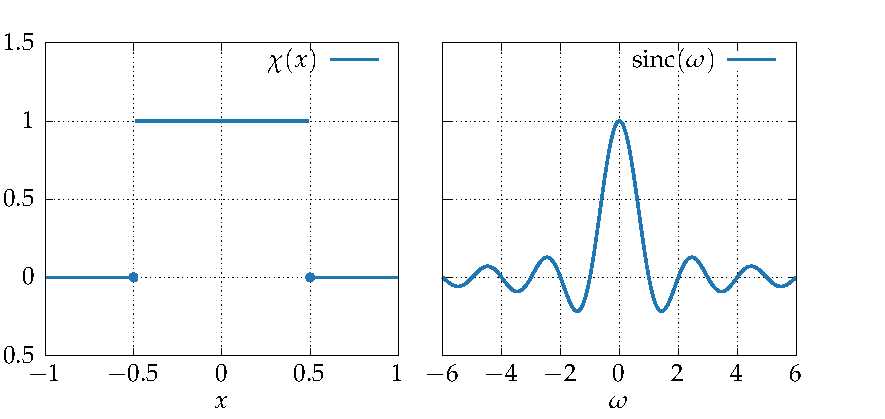
\includegraphics{gp_sinc-ft.pdf}
  \caption{This figure illustrates~\cref{ex:sinc-ft}. The indicator function of the
    interval $(-\frac{1}{2},\frac{1}{2})$ defined in~\cref{eq:int-indicator} is
    represented in the left pane. The right pane represents its Fourier transform, the
  sine cardinal function.}
  \label{fig:sinc-ft}
\end{figure}
\begin{example}
  \label{ex:sinc-ft}
  Let $\chi$ be the function on $\R$ defined by
  \begin{equation}
    \chi(x)=
    \begin{cases}
      1&\text{if}~-\frac{1}{2}<x<\frac{1}{2}\\
      0&\text{else}
    \end{cases}\,,
    \label{eq:int-indicator}
  \end{equation}
  for all $x\in\R$. $\chi$ is a rapidly decaying function, but it is not a Schwartz
  function as it has discontinuities at $-1$ and $1$. Its Fourier transform is given by
  \begin{equation}
    \hat{\chi}(\omega)=\int_{-\frac12}^{\frac12}\diff x\,e^{-2\pi i\omega x}=
    -\frac{1}{2\pi i\omega}(e^{-\pi i\omega}-e^{\pi i\omega})
    =\frac{\sin(\pi\omega)}{\pi\omega}\,.
  \end{equation}
  The function $\hat{\chi}(\omega)$ is called the \emph{sine cardinal function} and is
  generally noted $\sinc$:
  \begin{equation}
    \sinc(x)=\frac{\sin(\pi x)}{\pi x}\,.
  \end{equation}
  Although this function has an apparent singularity at $x=0$, $\sin(\pi x)\simeq \pi x$
  for $x\to0$, therefore $\sinc$ can be continued to the finite value $\sinc(0)=1$. $\chi$
  and its Fourier transform are illustrated in~\cref{fig:sinc-ft}. We can observe that
  although $\chi$ is rapidly decaying, its Fourier transform is not. This is related to
  the lack of smoothness of $\chi$. As we will see below, this is not an issue with
  Schwartz functions.
\end{example}
As in the case of Fourier coefficients (\cref{prop:fourier-coef-trans}), the Fourier
transform admits some useful transformation identities. We start by defining the
conjugation and scaling operators.
\begin{definition}
  For any function $f$ on $\R$, we define the \emph{conjugation operator} $\mathcal{C}$
  which associates to $f$ its complex conjugate $\mathcal{C}f=f^*$.
\end{definition}
\begin{definition}
  For any function $f$ on $\R$, and any positive real number $\delta$, we define the
  \emph{scaling operator} $\mathcal{S}_{\delta}$ which associates to $f$ the function
  defined by $\mathcal{S}_{\delta}f(x)=f(\delta x)$, for all $x\in\R$.
\end{definition}
\begin{proposition}
  The conjugation, reflection, translation, and scaling of a Schwartz function are still
  Schwartz functions.
\end{proposition}
Then we have the following transformation rules.
\begin{proposition}
  \label{prop:ft-trans}
  Let $f$ be a Schwartz function on $\R$, the following properties hold
  \begin{enumerate}
    \item \emph{Conjugation}: $\mathcal{F}(f^*)(\omega)=[\hat{f}(-\omega)]^*$, or
      $\mathcal{F}\mathcal{C}=\mathcal{C}\mathcal{R}\mathcal{F}$.
    \item \emph{Reflection}: $\mathcal{F}(\tilde{f})(\omega)=\hat{f}(-\omega)$, or
      $\mathcal{F}\mathcal{R}=\mathcal{R}\mathcal{F}$.
    \item \emph{Translation}: For $a\in\R$, $(\mathcal{F}\mathcal{T}_{a})f(\omega)
      =e^{-2\pi i\omega a}\hat{f}(\omega)$, or
      $\mathcal{F}\mathcal{T}_{a}=\ew(-a)\mathcal{F}$.
    \item \emph{Scaling}: For $\delta\in\R$ with $\delta>0$,
      $(\mathcal{F}\mathcal{S}_{\delta})f(\omega)=\delta^{-1}\hat{f}(\delta^{-1}\omega)$,
      or
      $\mathcal{F}\mathcal{S}_{\delta}=\delta^{-1}\mathcal{S}_{\delta^{-1}}\mathcal{F}$.
    \item \emph{Differentiation in space:} For $\alpha$ a non-negative integer,
      $\mathcal{F}(f^{(\alpha )})=(2\pi i\omega)^{\alpha}\hat{f}(\omega)$.
    \item \emph{Differentiation in frequency:} For $\alpha$ a non-negative integer,
      $\hat{f}$ is $\alpha$ times differentiable. Let $g$ be the function defined for
      $x\in\R$ by $g(x)=(-2\pi ix)^\alpha f(x)$, then $\hat{g}=\hat{f}^{(\alpha)}$.
  \end{enumerate}
\end{proposition}
\begin{proof}
  The proof of this proposition is part of the exercises of this chapter.
\end{proof}
A first important property of Schwartz functions is that their decay and smoothness
properties are preserved by the Fourier transform:
\begin{theorem}
  If $f$ is a Schwartz function, then its Fourier transform $\hat{f}$ is also a Schwartz
  function.
\end{theorem}
\begin{proof}
  Let us first observe that the Fourier transform of a Schwartz function always goes to
  zero at infinity, which is a variant of the Riemann-Lebesgue lemma for Schwartz
  functions. Using \cref{prop:ft-trans}, we know that for $\omega\neq 0$,
  \begin{equation}
    \hat{f}(\omega)=\frac{1}{2\pi i\omega}\mathcal{F}(f')\,.\label{eq:ft-ip}
  \end{equation}
  Since $f'$ is a Schwartz function, its Fourier transform is bounded by
  \begin{equation}
    |\mathcal{F}(f')|=\left|\intr{x}f'(x)\,e^{-2\pi i \omega x}\right|\leq
    \intr{x}|f'(x)|\,,
  \end{equation}
  therefore taking $|\omega|\to+\infty$ in~\cref{eq:ft-ip}, we get
  \begin{equation}
    \lim_{|\omega|\to+\infty}\hat{f}(\omega)=0
  \end{equation}
  Now, let $\alpha$ and $\beta$ be two non-negative integers. Then, using
  \cref{prop:ft-trans}, for all $\omega\in\R$,
  \begin{equation}
    \omega^\beta\hat{f}^{(\alpha)}(\omega)
    =\frac{1}{(2\pi i)^{\beta}}\mathcal{F}(f^{(\alpha+\beta)})(\omega)\,.
  \end{equation}
  Since $f^{(\alpha+\beta)}$ is a Schwartz function (\cref{prop:schwartz-comb}), then as
  discussed above its Fourier transform goes to zero at infinity, and therefore
  \begin{equation}
    \lim_{|\omega|\to+\infty}\omega^\beta\hat{f}^{(\alpha)}(\omega)=0\,,
  \end{equation}
  which proves that $\hat{f}$ is a Schwartz function.
\end{proof}
Another important property is the Fourier transform of Gaussian kernels.
\begin{theorem}[Gaussian uncertainty principle]
  \label{thm:gauss-uncertainty}
  The Fourier transform of a Gaussian kernel of width $\sigma$ is, up to a proportionality
  factor, a Gaussian kernel of width $\hat{\sigma}=\frac{1}{2\pi\sigma}$:
  \begin{equation}
    \hat{\gauss}_{\sigma}(\omega)=
    \frac{1}{\sigma\sqrt{2\pi}}\gauss_{\hat{\sigma}}(\omega)
    =e^{-2\pi^2\sigma^2\omega^2}\,.
  \end{equation}
  In particular,
  \begin{equation}
    \sigma\hat{\sigma}=\frac{1}{2\pi}\,.\label{eq:gauss-uncertainty}
  \end{equation}
\end{theorem}
\begin{proof}
  The proof of this proposition is part of the exercises of this chapter.
\end{proof}
The theorem above is called the ``uncertainty principle'' in reference to the original
work of physicist Werner Heisenberg in quantum mechanics, where this relationship was
first observed. However, it is important to note that it has a wide range of implications
and interpretations beyond quantum mechanics. The general interpretation is that if the
resolution of an object in space is dictated by a Gaussian distribution of a given width,
then the associated distribution in frequency has the inverse width. A direct consequence
is that it is impossible to achieve arbitrarily high resolution both in space and
frequency simultaneously, hence the ``uncertainty''.
%-----------------------------------------------------------------------------------------
\subsection{Convolution product}
A key operation in Fourier analysis is the \emph{convolution product}. When convoluting a
function $f$ by another function $g$, one averages from a given point $x$ the values of
$f$ according to the weights given by $g$:
\begin{definition}
  Let $f$ and $g$ be two functions on $\R$ such that the integral
  \begin{equation}
    (f\ast g)(x)=\intr{y}f(x-y)g(y)\label{eq:conv-def}
  \end{equation}
  is well-defined and finite for all $x\in\R$. The function $f\ast g$ defined on $\R$ by
  the relation above is called the \emph{convolution product} of $f$ and $g$. The
  convolution product can also be written as the dot product
  \begin{equation}
    (f\ast g)(x)=\braket{\mathcal{R}\mathcal{T}_xf,g^*}\,.
  \end{equation}
\end{definition}
Convolution products are bilinear and commutative:
\begin{proposition}
  Let $f$, $g$ and $h$ be three functions on $\R$ such that $f\ast g$ and $f\ast h$ are
  well-defined. Then,
  \begin{equation}
    f\ast g=g\ast f\,,
  \end{equation}
  and for all pairs of complex numbers $a$, $b$,
  \begin{equation}
    f\ast (ag+bh)=a(f\ast g) + b(f\ast h)\,.
  \end{equation}
\end{proposition}
\begin{proof}
  The commutation property is obtained by using the change of variable $z=x-y$ in the
  definition \cref{eq:conv-def}. The second formula is a trivial consequence of the
  integral linearity.
\end{proof}
Convolution products have crucial regularisation properties. Roughly speaking, a product
$f\ast g$ will have the smoothness properties of the smoothest function between $f$ and
$g$. In particular, convoluting by a Schwartz function leads to a smooth function:
\begin{theorem}
  Let $f$ be a Schwartz function on $\R$ and $g$ be an integrable moderately growing
  function on $\R$. The convolution product $f\ast g$ is an infinitely differentiable
  moderately growing function and for all non-negative integers $\alpha$,
  \begin{equation}
    (f\ast g)^{(\alpha)}=f^{(\alpha)}\ast g\,.
  \end{equation}
\end{theorem}
\begin{proof}
  The function $F$ defined on $\R^2$ by
  \begin{equation}
    F(x,y)=f(x-y)g(y)\,,
  \end{equation}
  is rapidly decaying in $y$, and its derivative in $x$ is also rapidly decaying in $y$.
  One can show that under these conditions\footnote{This is the Leibniz integral rule,
  \cf\cref{ft-trans}}, the integral of $F$ in $y$ is differentiable in $x$, and that the
  derivative and integral can be exchanged. This leads to
  \begin{equation}
    (f\ast g)'(x)=\frac{\diff}{\diff x}\intr{y}f(x-y)g(y)
    =\intr{y}f'(x-y)g(y)=(f'\ast g)(x)\,,
  \end{equation}
  and the result of the theorem can be obtained by repeating the operation above $\alpha$
  times. We will admit the fact that $f\ast g$ is a moderately growing function.
  Intuitively, since $f$ decays fast, it cannot accelerate the growth of $g$ through the
  convolution product.
\end{proof}
In general, $f\ast g$ inherits from the worse decay rate between $f$ and $g$. The theorem
above can be specialised for Schwartz functions, which we will admit here:
\begin{proposition}
  Let $f$ and $g$ be two Schwartz functions, then $f\ast g$ is a Schwartz function.
\end{proposition}
A crucial form of convolution is to convolute a function by a Gaussian kernel. Under
favourable conditions, it generates an arbitrarily good smooth approximation of the
function as the Gaussian width goes to zero, as discussed below.
\begin{theorem}
  \label{thm:gaussian-unit}
  Let $f$ be a moderately growing function on $\R$, continuous at a point $x\in\R$. Then,
  \begin{equation}
    \lim_{\sigma\to 0}(f\ast \gauss_{\sigma})(x)=f(x)\,.
  \end{equation}
\end{theorem}
\begin{proof}
  We write
  \begin{equation}
    (f\ast \gauss_{\sigma})(x)=\intr{y}f(x-y)\gauss_{\sigma}(y)\,.
  \end{equation}
  Changing the variable with $y=\sigma z$, we obtain
  \begin{equation}
    (f\ast \gauss_{\sigma})(x)=\intr{z}f(x-\sigma z)\gauss_{1}(z)\,.
  \end{equation}
  Admitting we can exchange limit and integral, and using the fact that $f$ is continuous,
  \begin{equation}
    \lim_{\sigma\to 0}(f\ast \gauss_{\sigma})(x)=f(x)\intr{z}\gauss_{1}(z)=f(x)\,.
  \end{equation}
  The exchange of the limit and integral can be shown to be a consequence of $f(x-\sigma
  z)\gauss_{1}(z)$ being rapidly decaying in $z$.
\end{proof}
\begin{corollary}
  \label{cor:gauss-sample}
  Let $f$ be a moderately growing function on $\R$ continuous in $0$, then
  \begin{equation}
    \lim_{\sigma\to0}\braket{f,\gauss_{\sigma}}=f(0)\,.
  \end{equation}
\end{corollary}
\begin{proof}
  One first observes that
  \begin{equation}
    (\tilde{f}\ast g)(x)=\intr{y}f(y-x)\gauss_{\sigma}(y)\,,
  \end{equation}
  therefore
  \begin{equation}
    \braket{f,\gauss_{\sigma}}=(\tilde{f}\ast g)(0)\,,
  \end{equation}
  which proves the corollary using~\cref{thm:gaussian-unit}.
\end{proof}
Finally, for Schwartz functions~\cref{thm:gaussian-unit} is uniformly convergent, which we
will admit.
\begin{theorem}
  Let $f$ be a Schwartz function on $\R$, then $f\ast \gauss_{\sigma}$ converges uniformly
  to $f$ for $\sigma\to 0$.
\end{theorem}
We conclude this section by an explicit example of Gaussian convolution.
\begin{figure}[t]
  \centering
  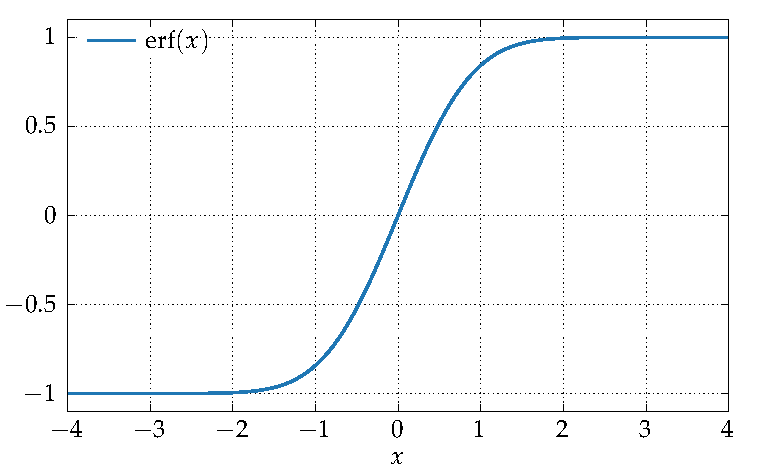
\includegraphics{gp_erf.pdf}
  \caption{Curve of the error function defined in~\cref{eq:erf}.}
  \label{fig:erf}
\end{figure}
\begin{figure}[htbp]
  \centering
  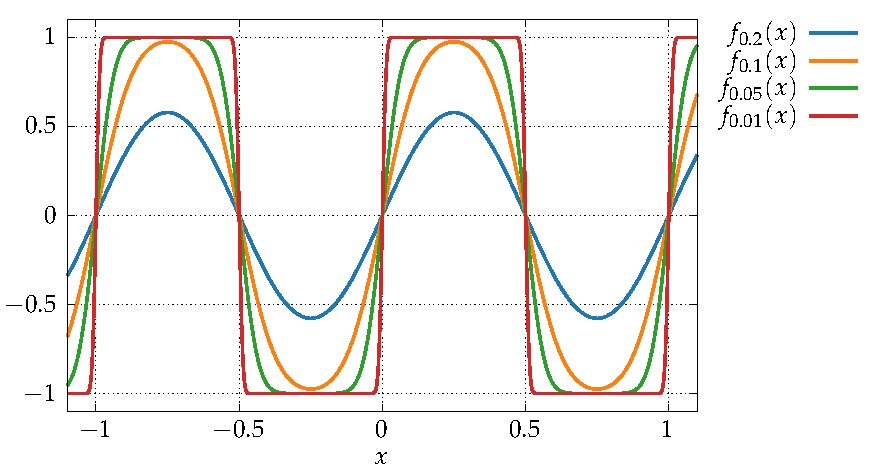
\includegraphics{gp_sq-gauss.pdf}
  \caption{Curve of the Gaussian-smoothed square wave
  in~\cref{eq:sq-gauss,eq:sq-gauss-exp} with smoothing widths from $0.2$ to $0.01$.}
  \label{fig:sq-gauss}
\end{figure}
\begin{example}
  For a positive real number $\sigma$, we define the following regularisation of the
  square wave using a Gaussian convolution:
  \begin{equation}
    f_\sigma=\sq\ast\gauss_\sigma\,.\label{eq:sq-gauss}
  \end{equation}
  Let us evaluate $f_\sigma$ explicitly. We first define the indicator function
  $\chi(a,b)$ of the interval $[a,b)$, where $a$ and $b$ are two real numbers such that
  $a<b$:
  \begin{equation}
    \chi(a,b)(x)=
    \begin{cases}
      1&\text{if}~a\leq x<b\\
      0&\text{otherwise}
    \end{cases}\,.
  \end{equation}
  The square wave can then clearly be written as an alternating sum of such functions:
  \begin{equation}
    \sq=\sumz{n}(-1)^{n}\chi\left(\frac{n}{2},\frac{n+1}{2}\right)\,.
    \label{eq:sq-chi-series}
  \end{equation}
  The series above is clearly convergent since only one term in the sum is non-zero at a
  given point. Then, for $x\in\R$
  \begin{equation}
    [\chi(a,b)\ast\gauss_\sigma](x)=\intr{y}\chi(a,b)(x-y)\gauss_\sigma(y)
    =\frac{1}{\sigma\sqrt{2\pi}}\int_{x-b}^{x-a}\diff y\,e^{-\frac{y^2}{2\sigma^2}}\,.
    \label{eq:chi-gauss}
  \end{equation}
  The integral above cannot be simplified much further, and is generally standardised
  through the \emph{error function} defined for $x\in\R$ by
  \begin{equation}
    \erf(x)=\frac{2}{\sqrt{\pi}}\int_0^x\diff y\,e^{-y^2}\,.\label{eq:erf}
  \end{equation}
  The error function is odd and converges quickly to $\pm 1$ as $x$ approaches
  $\pm\infty$. It is illustrated in~\cref{fig:erf}. Its name comes from its relevance to
  error estimation of quantities following Gaussian statistics. Now, using the change of
  variable $z=\frac{y}{\sigma\sqrt{2}}$ in~\cref{eq:chi-gauss},
  \begin{equation}
    [\chi(a,b)\ast\gauss_\sigma](x)=\frac{1}{\sqrt{\pi}}
    \int_{\frac{x-b}{\sigma\sqrt{2}}}^{\frac{x-a}{\sigma\sqrt{2}}}\diff z\,e^{-z^2}
    =\frac{1}{2}\left[\erf\left(\frac{x-b}{\sigma\sqrt{2}}\right)
    -\erf\left(\frac{x-a}{\sigma\sqrt{2}}\right)\right]\,.
  \end{equation}
  Using this expression with~\cref{eq:sq-chi-series}, we obtain
  \begin{equation}
    f_\sigma=\frac{1}{2}\sumz{n}(-1)^{n}
    \left[\erf\bigg(\frac{x-\frac{n+1}{2}}{\sigma\sqrt{2}}\bigg)
    -\erf\bigg(\frac{x-\frac{n}{2}}{\sigma\sqrt{2}}\bigg)\right]\,.
    \label{eq:sq-gauss-exp}
  \end{equation}
  The result above is represented in~\cref{fig:sq-gauss}.
\end{example}
We now have the required tools to investigate the inversion of the Fourier transform
conjectured in~\cref{eq:ft-conjecture}, which is the topic of the next section.
%-----------------------------------------------------------------------------------------
\subsection{Inverse Fourier transform}
We start by discussing a fundamental identity of Fourier analysis.
\begin{theorem}
  \label{thm:fourier-adj}
  Let $f$ and $g$ be two Schwartz functions on $\R$, then
  \begin{equation}
    \intr{\omega}\hat{f}(\omega)g(\omega)=\intr{x}f(x)\hat{g}(x)\,.
  \end{equation}
\end{theorem}
\begin{proof}
  We consider the function $F$ on $\R^2$ defined by
  \begin{equation}
    F(x,\omega)=f(x)g(\omega)\,e^{-2\pi i\omega x}\,.
  \end{equation}
  Because of the rapid decay of $F$ in $x$ and $\omega$, $|F(x,\omega)|$ has a
  well-defined two-dimensional integral on $x$ and $\omega$. One can show that under these
  conditions, the one-dimensional integrals on $x$ and $\omega$ can be performed in any
  order\footnote{This result is known as \emph{Fubini's theorem}.}, which proves the
  theorem.
\end{proof}
Using the previous theorem with~\cref{thm:gauss-uncertainty} allow to prove the Fourier
inversion conjectured in~\cref{eq:ft-conjecture} for Schwartz functions, which is one of
the main result of this chapter.
\begin{theorem}[Fourier inversion]
  \label{thm:fourier-inv}
  Let $f$ be a Schwartz function on $\R$, then for all $x\in\R$,
  \begin{equation}
    f(x)=\intr{\omega}\hat{f}(\omega)\,e^{2\pi i\omega x}\,.
  \end{equation}
  In other words, the Fourier transform is an invertible operation, and
  $\mathcal{F}^{-1}=\mathcal{R}\mathcal{F}=\mathcal{F}\mathcal{R}$.
\end{theorem}
\begin{proof}
  Let $\sigma$ be a positive real number. We define the function $G$ on $\R$ with
  \begin{equation}
    G(\omega)=e^{-4\pi^2\sigma^2\omega^2}
    =\frac{1}{\sigma\sqrt{2\pi}}\gauss_{\frac{1}{2\pi\sigma}}(x)\,.
  \end{equation}
  $g$ is clearly a Schwartz function, and according to~\cref{thm:gauss-uncertainty}, its
  Fourier transform is given by
  \begin{equation}
    \hat{G}=\frac{1}{\sigma\sqrt{2\pi}}\,\hat{\gauss}_{\frac{1}{2\pi\sigma}}
    =\gauss_{\sigma}\,.
  \end{equation}
  For a given $y\in\R$, we additionally define the function $F$ for all $x\in\R$ with
  \begin{equation}
    F(x)=f(x+y)=(\mathcal{T}_{-y}f)(x)\,.
  \end{equation}
  According to~\cref{prop:ft-trans}, the Fourier transform of $F$ is given by
  \begin{equation}
    \hat{F}(\omega)=e^{2\pi i\omega y}\hat{f}(\omega)\,.
  \end{equation}
  Now, using, using~\cref{thm:fourier-adj},
  \begin{equation}
    \intr{\omega}\hat{F}(\omega)G(\omega)=\intr{x}F(x)\hat{G}(x)\,.
  \end{equation}
  Using the change of variable $z=-x$ in the right-hand side of the equation above, and
  the fact that $\hat{G}$ is even, one obtains
  \begin{equation}
    \intr{x}F(x)\hat{G}(x)=\intr{x}f(y-x)\hat{G}(x)=(f\ast\hat{G})(y)
    =(f\ast\gauss_{\sigma})(y)\,.
  \end{equation}
  Therefore, using~\cref{thm:gaussian-unit},
  \begin{equation}
    \lim_{\sigma\to 0}\intr{x}F(x)\hat{G}(x)=f(y)\,,
  \end{equation}
  uniformly. Finally,
  \begin{equation}
    \lim_{\sigma\to 0}\intr{\omega}\hat{F}(\omega)G(\omega)=
    \intr{\omega}\hat{F}(\omega)=\intr{\omega}\hat{f}(\omega)\,e^{2\pi i\omega y}\,,
  \end{equation}
  which proves the theorem. We did not completely justify the exchange of limit and
  integral in this last step, and it can be shown to be a consequence of the
  \emph{dominated convergence theorem}.
\end{proof}
The Fourier inversion theorem can be easily reformulated as a set of operator identities.
Essentially, from an operator point of view, the Fourier transform is a square root of the
reflection operation, and a fourth root of the identity.
\begin{corollary}
  \label{cor:ft-id}
  We have the following identities
  \begin{equation}
    \mathcal{F}^2=\mathcal{R}\qquad\text{and}\qquad\mathcal{F}^4=1\,,
  \end{equation}
  \ie two successive Fourier transforms are equivalent to a reflection, and four
  successive Fourier transforms cancel each other. Additionally, if $f$ and $g$ are two
  Schwartz functions,
  \begin{equation}
    \braket{\mathcal{F}f,g}=\braket{f,\mathcal{F}^{-1}g}\,.
  \end{equation}
\end{corollary}
\begin{proof}
  Using~\cref{prop:ft-trans,thm:fourier-inv},
  $\mathcal{F}^{-1}=\mathcal{R}\mathcal{F}=\mathcal{F}\mathcal{R}$, so
  $\mathcal{F}^2=\mathcal{R}$. Clearly two successive reflections cancel each other, \ie
  $\mathcal{R}^2=1$, so $\mathcal{F}^4=1$. Finally,
  using~\cref{thm:fourier-adj,prop:ft-trans},
  \begin{align}
    \braket{\mathcal{F}f,g}&=\intr{\omega}\hat{f}(\omega)g(\omega)^*
    =\intr{x}f(x)\mathcal{F}(g^*)(x)\\
    &=\intr{x}f(x)[(\mathcal{R}\mathcal{F}g)(x)]^*
    =\intr{x}f(x)[(\mathcal{F}^{-1}g)(x)]^*\\
    &=\braket{f,\mathcal{F}^{-1}g}\,.
  \end{align}
\end{proof}
The previous identities lead to Plancherel's theorem, which is the generalisation of
Parseval's theorem (\cref{thm:parseval}) for Fourier transforms.
\begin{theorem}[Plancherel]
  Let $f$ be a Schwartz function on $\R$, then $\|f\|=\|\hat{f}\|$.
\end{theorem}
\begin{proof}
  Using~\cref{cor:ft-id},
  \begin{equation}
    \|\hat{f}\|^2=\braket{\mathcal{F}f,\mathcal{F}f}
    =\braket{f,\mathcal{F}^{-1}\mathcal{F}f}
    =\braket{f,f}=\|f\|^2\,.
  \end{equation}
\end{proof}
We conclude this section with a crucial identity in Fourier analysis: the
\emph{convolution theorem}. The Fourier transform maps a convolution product into a
regular multiplication, which can considerably simplify the practical computation of
convolutions.
\begin{theorem}[Convolution theorem]
  Let $f$ and $g$ be two Schwartz functions on $\R$, then
  \begin{equation}
    \mathcal{F}(f\ast g)=\hat{f}\,\hat{g}\qquad\text{and}\qquad
    \mathcal{F}(fg)=\hat{f}\ast\hat{g}\,.
  \end{equation}
\end{theorem}
\begin{proof}
  The proof of this theorem is similar the proof of~\cref{thm:fourier-adj}. For
  $\omega\in\R$, we define the function
  \begin{equation}
    F(x,y)=f(x-y)g(y)e^{-2\pi i \omega x}\,,
  \end{equation}
  and clearly
  \begin{equation}
    \intr{x}\intr{y}F(x,y)=\mathcal{F}(f\ast g)(\omega)\,.
  \end{equation}
  It can be shown that since $f$ and $g$ are both rapidly decaying, the integrals on $x$
  and $y$ above can be performed in any order. Using~\cref{prop:ft-trans}, integrating
  first on $x$ leads to
  \begin{equation}
    \intr{x}F(x,y)=\hat{f}(\omega)g(y)e^{-2\pi i\omega y}\,,
  \end{equation}
  then integrating on $y$ proves $\mathcal{F}(f\ast g)=\hat{f}\,\hat{g}$. The second
  identity is obtained through
  \begin{equation}
    \mathcal{F}(\hat{f}\ast\hat{g})=\mathcal{R}(fg)\,,
  \end{equation}
  where we used $\mathcal{F}^2=\mathcal{R}$ (\cref{cor:ft-id}), and the trivial identity
  $\mathcal{R}(fg)=(\mathcal{R}f)(\mathcal{R}g)$. Then
  \begin{equation}
    \hat{f}\ast\hat{g}=\mathcal{F}^{-1}\mathcal{R}(fg)=\mathcal{F}\mathcal{R}^2(fg)
    =\mathcal{F}(fg)\,.
  \end{equation}
\end{proof}
The convolution theorem also offers another interpretation of the smoothing properties of
convolution products. If a function $f$ is convoluted with a smooth function $g$, then the
Fourier transform $\hat{f}$ is simply multiplied by $\hat{g}$. Since $g$ is smooth,
$\hat{g}$ decays fasts, then the product $\hat{f}\hat{g}$ also decays fast, which in turn
means that the convolution product is indeed smooth.

As we discussed in this section, Schwartz functions have good properties regarding the
Fourier transform. The Fourier transform acts as a one-to-one mapping of Schwartz
functions onto themselves, with a simple inversion formula. The Schwartz functions are
also stable under key Fourier analysis operations such as convolution products,
differentiation, and multiplication by powers. However, a large volume of functions
relevant to physical problems are not Schwartz functions, and some generalisation is
needed. There are multiple ways to extend the Fourier transform to more general classes of
functions. In the next section, we will focus on the construction which is implicitly the
underlying one in most physical applications.
%%%%%%%%%%%%%%%%%%%%%%%%%%%%%%%%%%%%%%%%%%%%%%%%%%%%%%%%%%%%%%%%%%%%%%%%%%%%%%%%%%%%%%%%%%
\section{Distributions -- \textit{There be dragons}} A key challenge in constructing the
Fourier transform is to ensure we can properly define its inverse. We showed in the
previous section that it is well understood for Schwartz functions. However, for
non-smooth functions, the Fourier transform decays slowly, as illustrated
in~\cref{ex:sinc-ft}. This lead to issues for defining an inverse transform. As we discuss
in this section, defining the Fourier transform more widely generally requires
generalising the concept of function itself, leading to objects called
\emph{distributions} or \emph{generalised functions}. Such ideas were used heuristically
in physical problems in the early 20\textsuperscript{th} for solving partial differential
equations, and notoriously by Paul Dirac in the early days of quantum physics. Those ideas
were then developed into a more justified mathematical framework, particularly by Sergei
Sobolev and Laurent Schwartz in the 1930s and 1940s. The theory of distributions is an
advanced mathematical topic, however it is a crucial tool for formulating modern physics.
Therefore, this section is mainly aimed at being a heuristic and practical introduction
for physics students, rather than an accurate description of the theory.

Let us start with the simple question: what should the Fourier transform of the constant
function equal to $1$ be? $1$ is neither decaying nor integrable, and the previous
construction based on Schwartz functions does not apply. For the moment, let us assume
that such an object exists and that we can define the Fourier transform $u=\hat{1}$.
Intuitively, $u(\omega)$ is the component of frequency $\omega$ of $1$. The function $1$
is a zero-frequency elementary wave, so we expect $u(\omega)=0$ for all $\omega\neq 0$ and
$u(0)$ to have some non-zero value to be determined. We also would like the duality
between the Fourier transform and its inverse $\mathcal{F}^{-1}=\mathcal{R}\mathcal{F}$ to
be preserved, and a key component in establishing that was~\cref{thm:fourier-adj}.
Assuming this formula, one would obtain
\begin{equation}
  \intr{\omega}u(\omega)\varphi(\omega)=\intr{x}\hat{\varphi}(x)=\varphi(0)\,,
  \label{eq:one-ft}
\end{equation}
for any Schwartz function $\varphi$. Another way to try defining $u$ is to define $1$ as
the limit of a sequence of Schwartz functions, for which the Fourier transform is
well-defined. For example, defining
\begin{equation}
  f_{\sigma}(x)=e^{-2\pi^2\sigma^2 x}\,,
\end{equation}
clearly $f_\sigma\to 1$ for $\sigma\to 0$. Additionally, according to
\cref{thm:gauss-uncertainty}, we know that the Fourier transform of $f_{\sigma}$ is just
the Gaussian kernel of width $\sigma$:
\begin{equation}
  \hat{f}_{\sigma}(\omega)=\gauss_\sigma(\omega)=\frac{1}{\sigma\sqrt{2\pi}}\,
  e^{-\frac{\omega^2}{2\sigma^2}}\,.
\end{equation}
We can try to define $u$ as the limit of $\hat{f}_{\sigma}$ for $\sigma\to 0$, which leads
to
\begin{equation}
  u(\omega)=\lim_{\substack{\sigma\to 0\\\sigma>0}}\,\hat{f}_{\sigma}(\omega)=
  \begin{cases}
    +\infty&\text{if}~\omega=0\\
    0&\text{else}
  \end{cases}\,.
\end{equation}
Although the result above is quite singular, this is essentially what is expected: the
function $1$ is composed only of a zero-frequency wave, by an infinite amount since we are
considering an infinite range. Unfortunately, this is inconsistent with~\cref{eq:one-ft}.
Indeed, $u$ as defined above is zero everywhere except at one point, which means that
\begin{equation}
  \intr{\omega}u(\omega)\varphi(\omega)=0\,,
\end{equation}
for any Schwartz function $\varphi$, which clearly contradicts~\cref{eq:one-ft}. However,
there is no contradiction if we keep the $\sigma\to 0$ limit \emph{outside} the integral:
\begin{equation}
  \lim_{\sigma\to 0}\intr{\omega}\hat{f}_{\sigma}(\omega)\varphi(\omega)=\varphi(0)\,,
\end{equation}
which is~\cref{cor:gauss-sample}. In summary, we managed to form a consistent picture that
$u$ should satisfy~\cref{eq:one-ft}, which can be built from a limit of Schwartz functions
using Gaussian kernels. Nonetheless, we did not manage to properly define $u$ itself as a
function. One can argue that this could be due to arbitrary choices made in the procedure
above, however one can show that there exists no function that satisfies~\cref{eq:one-ft}:
\begin{proposition}
  \label{prop:delta-nogo}
  There exists no function $f$ that satisfies the equation
  \begin{equation}
    \intr{x}f(x)\varphi(x)=\varphi(0)\,,
  \end{equation}
  for all Schwartz functions $\varphi$.
\end{proposition}
\begin{proof}
  Let us assume that such a function $f$ exists. We first consider the \emph{bump
  function}
  \begin{equation}
    \varphi_A(x)=
    \begin{cases}
      \exp(-\frac{A^2}{A^2-x^2})&\text{if}~-A<x<A\\
      0&\text{else}
    \end{cases}\,,
  \end{equation}
  where $A$ is a positive real number. One can show that $\varphi_A$ is a Schwartz
  function, and it is smaller than $1$ in the $(-A,A)$ interval and zero everywhere else.
  On the one hand
  \begin{equation}
    \intr{x}f(x)\varphi_A(x)=\varphi_A(0)=e^{-1}\neq 0\,,
    \label{eq:int-dfn-bump}
  \end{equation}
  on the other hand,
  \begin{equation}
    \left|\intr{x}f(x)\varphi_A(x)\right|\leq\int_{-A}^A\diff x\,|f(x)|\,,
  \end{equation}
  which implies that
  \begin{equation}
    \lim_{A\to 0}\intr{x}f(x)\varphi_A(x)=0\,.
  \end{equation}
  This last equation contradicts~\cref{eq:int-dfn-bump}, which proves the proposition by
  contradiction.
\end{proof}
The previous proposition naively suggests that there is no solution to the problem
discussed. Another possible interpretation is that to define the Fourier transform of $1$,
one needs to generalise the concept of function to objects that can satisfy, in a sense to
be defined, the equation in \cref{prop:delta-nogo}.
%-----------------------------------------------------------------------------------------
\subsection{Definition of distributions}
A key observation we made in the previous introduction of this section is that computing
the Fourier transform of $1$ appears to lead to consistent results as long as expressions
are integrated against a Schwartz function. This allows us to define a new class of
mathematical objects, called \emph{distributions}\footnote{The specific distributions
  discussed here are more precisely called \emph{tempered distributions}; the term
\emph{generalised function} is also used in the literature.}:
\begin{definition}
  A \emph{distribution} $F$ on $\R$ is a linear operation that associates any to any
  Schwartz function $\varphi$ a complex number $F(\varphi)$. Explicitly, for any pair of
  Schwartz function $\varphi,\psi$ and any pair of complex numbers $a,b$,
  \begin{equation}
    F(a\varphi+b\psi)=aF(\varphi)+bF(\psi)\in\C\,.
  \end{equation}
  The value $F(\varphi)$ might be abusively written as an integral
  \begin{equation}
    F(\varphi)=\intr{x}F(x)\varphi(x)\,,
  \end{equation}
  and it is important to stress that on its own $F(x)$ is ill-defined, only its integral
  against a Schwartz function is properly defined.
\end{definition}
Distributions generalise the concept of moderately growing function through the following
definition and proposition.
\begin{definition}
  If $f$ is a moderately growing function on $\R$, then $f$ defines a distribution,
  abusively also noted $f$, using the dot product
  \begin{equation}
    f(\varphi)=\braket{f,\varphi^*}=\intr{x}f(x)\varphi(x)\,,
  \end{equation}
  for all Schwartz functions $\varphi$. Two moderately growing functions $f$ and $g$ are
  said to be equal \emph{in the sense of distributions} if $f(\varphi)=g(\varphi)$ for all
  Schwartz functions.
\end{definition}
\begin{proposition}
  If two Schwartz function are equal in the sense of distributions, they are also equal as
  functions. Explicitly, if $f$ and $g$ are two Schwartz functions such that
  \begin{equation}
    \intr{x}f(x)\varphi(x)=\intr{x}g(x)\varphi(x)\,,
  \end{equation}
  for all Schwartz functions $\varphi$, then $f=g$.
\end{proposition}
\begin{proof}
  This is a direct consequence of~\cref{thm:gaussian-unit}. For $y\in\R$, if one chooses
  \begin{equation}
    \varphi(x)=\gauss_{\sigma}(y-x)\,,
  \end{equation}
  then
  \begin{equation}
    0=\lim_{\sigma\to 0}\intr{x}[f(x)-g(x)]\gauss_{\sigma}(y-x)=
    \lim_{\sigma\to 0}[(f-g)\ast\gauss_{\sigma}](y)=f(y)-g(y)\,,
  \end{equation}
  which implies that $f=g$.
\end{proof}
This can be extended further using~\cref{thm:gaussian-unit}, which we will not do
precisely here. Essentially, if two functions are equal in the sense of distributions,
they are equal where they are continuous. However, it is easy to see that equality in the
sense of distributions is weaker than the usual equality, since changing the value of one
point in a function does not modify an integral. Finally, we define the delta
distribution, which address the issue raised by~\cref{prop:delta-nogo}.
\begin{definition}
  \label{def:delta}
  The \emph{delta} distribution $\delta$, sometimes also called \emph{Dirac delta}, is
  defined by
  \begin{equation}
    \delta(\varphi)=\intr{x}\delta(x)\varphi(x)=\varphi(0)\,,
  \end{equation}
  for all Schwartz functions $\varphi$.
\end{definition}
In the literature $\delta$ is often abusively referred to as the ``delta function'',
however it is important to stress that it is in fact not a function, because
of~\cref{prop:delta-nogo}. In summary, functions define distributions, but not all
distributions are defined by a function. So distributions do constitute a more general
class of objects than functions.

We can now reformulate~\cref{cor:gauss-sample} as follows:
\begin{proposition}
  We have the following limit
  \begin{equation}
    \lim_{\sigma\to 0}\gauss_{\sigma}(x)=\delta(x)\,,
  \end{equation}
  in the sense of distributions.
\end{proposition}
The definitions above give an easier meaning to some limit issues discussed in the
introduction of this section. For example, for a Schwartz function $\varphi$, we can now
write
\begin{equation}
  \lim_{\sigma\to 0}\intr{x}\gauss_{\sigma}(x)\varphi(x)=\intr{x}\delta(x)\varphi(x)
  =\varphi(0)\,.
\end{equation}
In other words, although the limit and integral above could not be exchanged in the
traditional sense, they can be exchanged in the sense of distributions.
%-----------------------------------------------------------------------------------------
\subsection{Distributional derivatives}
Many linear transformations on functions generalise well to distributions. One crucial and
important operation is to generalise the derivative to distributions:
\begin{definition}
  Let $F$ be a distribution on $\R$, then the derivative $F'$ is the distribution defined
  for all Schwartz functions $\varphi$ by
  \begin{equation}
    F'(\varphi)=-F(\varphi')\,,
  \end{equation}
  which can also be written
  \begin{equation}
    \intr{x}F'(x)\varphi(x)=-\intr{x}F(x)\varphi'(x)\,,
  \end{equation}
  which is simply a generalisation of integration by parts,
  \cf\cref{prop:schwartz-partint}.
\end{definition}
An interesting consequence of the definition above is that distributions allow to define
the derivative of discontinuous functions! One important case of such generalisation is
the \emph{Heaviside function}:
\begin{definition}
  We call \emph{Heaviside function}, also sometimes called \emph{theta function}, the
  function $\theta$ defined for all $x\in\R$ by
  \begin{equation}
    \theta(x)=
    \begin{cases}
      1&\text{if}~x\geq 0\\
      0&\text{else}
    \end{cases}\,.
  \end{equation}
\end{definition}
We can show that the derivative of the Heaviside function is in fact the delta function.
\begin{proposition}
  In the sense of distributions,
  \begin{equation}
    \theta'(x)=\delta(x)\,.
  \end{equation}
\end{proposition}
\begin{proof}
  Let $\varphi$ be a Schwartz function. Then:
  \begin{equation}
    \theta'(\varphi)=-\intr{x}\theta(x)\varphi'(x)=\int_0^{+\infty}\varphi'(x)
    =\varphi(0)=\delta(\varphi)\,,
  \end{equation}
  which proves the proposition.
\end{proof}
This last result is quite intuitive: the Heaviside function is flat everywhere, and has an
``infinite slope'' at zero because of the discontinuity, hence its derivative is the delta
function. As a final example, we can also compute the derivative of the delta function
\begin{equation}
  \intr{x}\delta'(x)\varphi(x)=-\intr{x}\delta(x)\varphi'(x)=-\varphi'(0)\,,
\end{equation}
and in general,
\begin{equation}
  \intr{x}\delta^{(n)}(x)\varphi(x)=(-1)^n\varphi^{(n)}(0)\,.
\end{equation}
%-----------------------------------------------------------------------------------------
\subsection{Transforming distributions}
Linear transformations previously introduced on functions generalise identically to
distributions, \ie conjugation, reflection, scaling, and translation. Changes of variable
in distributional integral also work identically to standard functions. We will not give
here the formal definitions. Instead, we will mainly discuss those transformations in the
context of examples involving the delta function.

Let $\varphi$ be a Schwartz function. Regarding translations, the statement above leads to
the formula
\begin{equation}
  \intr{x}\delta(x-a)\varphi(x)=\varphi(a)\,,
\end{equation}
where $a\in\R$. The equality above comes from using the change of variable $y=x+a$ and the
definition of the delta function. Another possible observation is that $\delta$ is even,
indeed,
\begin{equation}
  \intr{x}\delta(-x)\varphi(x)=\intr{x}\delta(y)\varphi(-y)=\varphi(0)\,,
\end{equation}
with $y=-x$, so
\begin{equation}
  \delta(-x)=\delta(x)\,,
\end{equation}
in the sense of distributions. We can similarly look at scaling, \ie
\begin{equation}
  \intr{x}\delta(ax)\varphi(x)=\frac{1}{|a|}\intr{x}\delta(y)\varphi(a^{-1}y)
  =\frac{\varphi(0)}{|a|}\,,
\end{equation}
with $y=ax$, and we assumed that $a\neq 0$. This leads to the distribution equality
\begin{equation}
  \delta(ax)=\frac{1}{|a|}\delta(x)\,.
\end{equation}

A more complicated question is whether we can combine $\delta$ with other functions. It
can be show that if $f$ is a moderately growing function continuous in $a\in\R$, one has
the following equality
\begin{equation}
  \label{eq:delta-times-f}
  \delta(x-a)f(x)=\delta(x-a)f(a)\,,
\end{equation}
in the sense of distributions. Approximating $\delta$ by a Gaussian kernel, this last
equation can be seen as a reformulation of \cref{cor:gauss-sample}. Defining the product
above if $f$ is discontinuous, or generally a distribution, is a highly non-trivial
problem. In general, it is well-defined to multiply distributions by smooth functions,
however multiplying distributions with distributions is ill-defined. It is a relevant
issue in some physical applications (\eg quantum field theory), but largely beyond the
scope of this course. It is also possible to define the convolution product for some
distributions. Some identities above, as well as~\cref{thm:gaussian-unit}, can be
reformulated as
\begin{equation}
  (f\ast\delta)(x)=f(x)\,,
\end{equation}
which is well-defined if $f$ is at least continuous. This last identity is important, as
it shows that the delta function is essentially a unit for the convolution product,
and~\cref{prop:delta-nogo} implies that there exists no standard function that fit that
requirement. Finally, we can look into composing a distribution with a function. This can
be generally defined through the change of variable formula, although the exact definition
can be quite technical. Let $u$ be a smooth and invertible function on $\R$ such that the
derivative of $u$ never cancels on $\R$. Then there is a unique point $x_0\in\R$ such that
$u(x_0)=0$, and we can write
\begin{equation}
  \intr{x}\delta[u(x)]\varphi(x)=\intr{y}\delta(y)|(u^{-1})'(y)|\varphi[u^{-1}(y)]
\end{equation}
where used the change of variables $y=u(x)$. Since $u^{-1}[u(x)]=x$, the derivative of the
inverse $u^{-1}$ is given by
\begin{equation}
  (u^{-1})'(x)=\frac{1}{u'[u^{-1}(x)]}\,,
\end{equation}
and therefore
\begin{equation}
  \intr{x}\delta[u(x)]\varphi(x)=\frac{\varphi(x_0)}{|u'(x_0)|}\,.
\end{equation}
This result can be written as
\begin{equation}
  \delta[u(x)]=\frac{\delta(x-x_0)}{|u'(x_0)|}\,,
\end{equation}
in the sense of distributions. The formula above can be generalised to more general
functions. For example, if $f$ is a smooth function that has zeros according to a sequence
$x_n$, and additionally if the derivative $f'$ never cancels at $x_n$ for all $n$, then
one can show that
\begin{equation}
  \delta[f(x)]=\sum_n\frac{\delta(x-x_n)}{|f'(x_n)|}\,,
\end{equation}
which we admit here. Composition can also be defined even if $f'$ cancels on the zeros of
$f$, but the result generally depends on some arbitrary regularisation procedure. Let us
discuss a couple of examples of the composition formula above.
\begin{example}
  If $a$ is a non-zero real number, then
  \begin{equation}
    \delta(x^2-a^2)=\frac{1}{2|a|}[\delta(x-a)+\delta(x+a)]\,.
  \end{equation}
\end{example}
\begin{example}
  If $\omega$ is a non-zero real number, then
  \begin{equation}
    \delta[\sin(\omega x)]=\sumz{n}\frac{\delta(x-n\pi)}{|\cos(n\pi)|}=\sumz{n}\delta(x-n\pi)\,.
  \end{equation}
\end{example}

Finally, it is also useful to know how to multiply a smooth function $f$ by a derivative of
the delta function. In general, if $F$ is a distribution, then one has
the usual formula $(Ff)'=F'f+Ff'$. Indeed,
\begin{align}
  (Ff)'(\varphi)=\intr{x}[Ff]'(x)\varphi(x)&=-\intr{x}F(x)f(x)\varphi'(x)\notag\\
  &=-\intr{x}F(x)[(f\varphi)'(x)-f'(x)\varphi(x)]\notag\\
  &=\intr{x}[F'(x)f(x)+F(x)f'(x)]\varphi(x)\notag\\
  &=(F'f)(\varphi)+(Ff')(\varphi)\,.
\end{align}
By differentiating in $x$ on both sides of~\cref{eq:delta-times-f}, we therefore obtain
\begin{equation}
  \delta'(x-a)f(x)+\delta(x-a)f'(x)=\delta'(x-a)f(a)\,,
\end{equation}
which can be simplified as
\begin{equation}
  \label{eq:delta1-times-f}
  \delta'(x-a)f(x)=\delta'(x-a)f(a)-\delta(x-a)f'(a)\,.
\end{equation}
In general, using recursively the steps above, one obtains
\begin{equation}
  \label{eq:deltan-times-f}
  \delta^{(\alpha)}(x-a)f(x)
  =\sum_{j=0}^{\alpha}(-1)^j\binom{\alpha}{j}f^{(j)}(a)\delta^{(\alpha-j)}(x-a)\,,
\end{equation}
where $\binom{\alpha}{j}$ is the binomial coefficient
\begin{equation}
  \binom{\alpha}{j}=\frac{\alpha!}{j!(\alpha-j)!}\,.
\end{equation}
%-----------------------------------------------------------------------------------------
\subsection{Distributional Fourier transform}
As we have conjectured in the introduction of this section, the Fourier transform of a
distribution can be defined by generalising \cref{thm:fourier-adj}:
\begin{definition}
  Let $F$ be a distribution on $\R$. The Fourier transform $\hat{F}=\mathcal{F}F$ of $F$
  is the distribution defined for all Schwartz functions $\varphi$ by
  \begin{align}
    \hat{F}(\varphi)=F(\hat{\varphi})\,.
  \end{align}
  Additionally, we will abusively write
  \begin{equation}
    \hat{F}(\omega)=\intr{x}F(x)\,e^{-2\pi i \omega x}\,,
  \end{equation}
  which allows to rewrite the definition above as
  \begin{align}
    \intr{\omega}\hat{F}(\omega)\varphi(\omega)&=\intr{\omega}
    \intr{x}F(x)\,e^{-2\pi i \omega x}\varphi(\omega)\notag\\
    &=\intr{x}F(x)\hat{\varphi}(x)\,,
    \label{eq:fourier-adj-dist}
  \end{align}
  where the integral signs can be freely exchanged.
\end{definition}
A first important result is that the Fourier transform of a complex wave is a delta
function:
\begin{proposition}
  For all $\omega_0\in\R$, one has
  \begin{equation}
    \intr{x}e^{2\pi i (\omega_0-\omega)x}=\delta(\omega-\omega_0)
  \end{equation}
\end{proposition}
\begin{proof}
  Let $\varphi$ be a Schwartz function, then
  \begin{equation}
    \intr{\omega}\intr{x}e^{2\pi i (\omega_0-\omega)x}\varphi(\omega)=
    \intr{x}e^{2\pi i\omega_0x}\hat{\varphi}(x)=\varphi(\omega_0)\,.
  \end{equation}
\end{proof}
In particular, this last result justifies the expected formula
\begin{equation}
  \intr{x}\delta(x)=1\,.
\end{equation}
We now formulate the inversion theorem, which is a direct consequence of the Fourier
inversion theorem for Schwartz functions.
\begin{theorem}[Distributional Fourier inversion]
  Let $F$ be a distribution on $\R$. Then
  \begin{equation}
    (\mathcal{F}^2F)(-x)=F(x)\,,
  \end{equation}
  which can be equivalently written
  \begin{equation}
    F(x)=\intr{\omega}\hat{F}(\omega)\,e^{2\pi i\omega x}\,.
  \end{equation}
\end{theorem}
\begin{proof}
  Let $\varphi$ be a Schwartz function, then
  \begin{align}
    \intr{x}(\mathcal{F}^2F)(-x)\varphi(x)&=\intr{x}(\mathcal{F}^2F)(x)\varphi(-x)\notag\\
    &=\intr{x}\mathcal{F}F(x)\mathcal{F}^{-1}\varphi(x)\notag\\
    &=\intr{x}F(x)\varphi(x)\,,
  \end{align}
  where we used \cref{cor:ft-id}.
\end{proof}
If $f$ is a smooth moderately growing function on $\R$, the Fourier inversion can also
simply be written as
\begin{align}
  \intr{\omega}\hat{f}(\omega)\,e^{2\pi i\omega x}&=
  \intr{\omega}\intr{y}f(y)\,e^{2\pi i\omega (x-y)}\notag\\
  &=\intr{y}f(y)\,\delta(x-y)=f(x)\,.
\end{align}
One can also show that the known transformation properties of the Fourier transform for
Schwartz functions generalise identically to distributions.
\begin{proposition}
  The conjugation, reflection, translation, and scaling properties of~\cref{prop:ft-trans}
  generalise identically to distributions.
\end{proposition}
\begin{proof}
  Left as an exercise to the reader.
\end{proof}
Additionally, the crucial duality between derivatives and powers through the Fourier
transform generalises to distributions.
\begin{proposition}
  \label{prop:ft-der-distrib}
  Let $F$ be a distribution on $\R$. Then for all non-negative integers $\alpha$,
  \begin{equation}
    \mathcal{F}(F^{(\alpha)})(\omega)=(2\pi i\omega)^{\alpha}\hat{F}(\omega)\,,
  \end{equation}
  in the sense of distributions.
\end{proposition}
\begin{proof}
  Let $\varphi$ be a Schwartz function, then
  \begin{equation}
    \intr{\omega}\mathcal{F}(F^{(\alpha)})(\omega)\,\varphi(\omega)
    =(-1)^{\alpha}\intr{x}F(x)\hat{\varphi}^{(\alpha)}(x)\,.
  \end{equation}
  We know that $\hat{\varphi}^{(\alpha)}$ is the Fourier transform
  of the function defined
  by $(-2\pi i\omega)^\alpha\varphi(\omega)$ (\cf\cref{prop:ft-trans}), therefore
  \begin{equation}
    \intr{\omega}\mathcal{F}(F^{(\alpha)})(\omega)\,\varphi(\omega)=
    \intr{\omega}(2\pi i\omega)^\alpha\hat{F}(\omega)\varphi(\omega)\,,
  \end{equation}
  which proves the proposition.
\end{proof}
Generalising convolution products to the convolution of two distributions $F$ and $G$ is a
non-trivial task which we will not formulate in details. However, the convolution theorem
holds when this is possible, so in physics applications one generally considers that if
$\hat{F}\hat{G}$ is well-defined, then its Fourier transform is the convolution product
$F\ast G$.

Finally, we state important characterisations of the Fourier transforms of some classes of
standard functions, which we will admit here.
\begin{theorem}
  The following properties hold:
  \begin{enumerate}
    \item If $f$ is an integrable function (\ie $\intr{x}|f(x)|$ is finite), then
      $\hat{f}$ if continuous and decays to zero at infinity.
    \item If $f$ is a square-integrable function (\ie $\intr{x}|f(x)|^2$ is finite), then
      $\hat{f}$ is also square-integrable and the Plancherel theorem holds, explicitly
      \begin{equation}
        \intr{x}|f(x)|^2=\intr{\omega}|\hat{f}(\omega)|^2\,.
      \end{equation}
  \end{enumerate}
\end{theorem}
We conclude these section with some important examples
\begin{proposition}
  Let $P$ be the degree $N$ polynomial defined by
  \begin{equation}
    P(x)=\sum_{n=0}^Na_nx^n\,,
  \end{equation}
  for all $x\in\R$. The Fourier transform of $P$ is given by
  \begin{equation}
    \hat{P}(\omega)=\sum_{n=0}^N\frac{a_n}{(-2\pi i)^n}\,\delta^{(n)}(\omega)\,,
  \end{equation}
  in the sense of distributions.
\end{proposition}
\begin{proof}
  We have
  \begin{equation}
    \mathcal{F}^{-1}(\delta^{(n)})(x)=(-2\pi i x)^n\mathcal{F}^{-1}(\delta)=
    (-2\pi i x)^n\,,
  \end{equation}
  which implies the proposition by linearity.
\end{proof}
%-----------------------------------------------------------------------------------------
\subsection{Summary for the pragmatic physicist}
Distributions are rather abstract objects, which can obfuscate the elegance of the
formalism they provide. Their introduction was strongly motivated by physics problems
which appeared to be solvable through Fourier analysis despite clear convergence issues
with the Fourier transform integral form. In summary:
\begin{itemize}
  \item The derivative of any function is defined in the sense of distributions. This
    conveniently includes discontinuous functions. Derivatives at discontinuity points
    generally generate purely distributional contributions (\eg delta functions) that
    would be undefined with standard functions.
  \item Distributional derivatives obey standard differentiation formulae.
  \item The Fourier transform of any function is defined in the sense of distributions,
    even if the standard definition as an integral is manifestly divergent.
  \item The Fourier transform of a distribution has the same transformation properties as
    standard functions (\ie the properties in \cref{prop:ft-trans}).
  \item Inversion and convolution theorems also hold for distributions.
  \item The delta function $\delta(\omega-a)$ is the Fourier transform of the elementary
    wave $e^{2\pi i xa}$, which provides useful identities in wave physics that would be
    otherwise undefined with standard functions.
\end{itemize}
In short, manipulating expressions in the sense of distributions requires considerably
less care than with standard functions, and most well-known properties hold. In physics,
functional manipulations are generally implicitly assumed to be in the sense of
distributions, particularly in field theory or when solving partial differential
equations. Distributions are abstract objects that can generally not represent a measurable
quantity; however, they are convenient and flexible for intermediate steps in a physical
theory.

The most important caveat with distributions is that one has to be very careful when
multiplying distributions. Multiplying a distribution by a smooth function is always
well-defined, but multiplying distributions that have non-smooth behaviour at identical
points almost always requires an arbitrary regularisation to be defined. For example, the
square of the delta function is not a well-defined distribution on its own.

Another limitation of Fourier analysis is that it can only describe functions that have
moderate growth. Functions with rapid growth (\eg exponential growth) can be relevant in
physics, and will not have a well-defined Fourier transform, even in the sense of
distributions. As we will see in the next chapter, they can nevertheless be described
indirectly through analytical continuation.
